\section{Integral Dependence and Valuations}
In classical algebraic geometry curves were frequently studied by projecting them onto a line and regarding the curve as a (ramified) covering of the line. This is quite analogous to the relationship between a number field and the rational field, or rather between their rings of integers, and the common algebraic feature is the notion of integral dependence. In this chapter we prove a number of results about integral dependence. We also give a brief treatment of valuations.
\subsection{Integral Dependence}
Let $B$ be a ring, $A$ a subring of $B$. An element $x\in B$ is said to be \textbf{integral} over $A$ if $x$ is a root of a monic polynomial with coefficients in $A$, that is if $x$ satisfies an equation of the form $x^n+a_1x^{n-1}+\cdots+a_n=0$, where $a_i$ are elements of $A$. Clearly every element of $A$ is integral over $A$.
\begin{example}\em
Suppose $A=\mathbb{Z}$, $B=\mathbb{Q}$. If a rational number $x=r/s\in\mathbb{Q}$ is integral over $\mathbb{Z}$, where $r$ and $s$ has no common divisor, by definition there exists some $a_i\in\mathbb{Z}$ such that $r^n+a_1r^{n-1}s+\cdots +a_ns^n=0$, hence $s$ divides $r^n$ and therefore $x\in\mathbb{Z}$.
\end{example}
\begin{proposition}
The following are equivalent:\par
(i) $x\in B$ is integral over $A$;\par
(ii) $A[x]$ is a finitely generated $A$-module;\par
(iii) $A[x]$ is contained in a subring $C$ of $B$ such that $C$ is a finitely generated $A$-module;\par
(iv) There exists a faithful $A[x]$-module $M$ which is finitely generated as an $A$-module.
\end{proposition}
\begin{proof}
(i)$\Rightarrow$(ii): Suppose $x\in B$ is integral over $A$, then there exists some $a_i\in A$ such that $x^{n+r}=-(a_1x^{n+r-1}+\cdots+a_nx^r)$ for all $r\ge 0$, hence by induction we have $A[x]$ is generated by $1,x,\cdots,x^{n-1}$ as an $A$-module.\par
(ii)$\Rightarrow$(iii): Take $C=A[x]$.\par
(iii)$\Rightarrow$(iv): Take $M=C$, we show that $M$ is a faithful $A[x]$-module. Suppose $y\in\mathrm{Ann}(M)$, then $yM=0$ for all $m\in M$, in particular we have $y\cdot 1=y=0$, hence $M$ is a faithful module.\par
(iv)$\Rightarrow$(i): Take $\phi$ to be the multiplication by $x$, and $\mathfrak{a}=A$, we have $xM\subset M$ since $M$ is an $A[x]$-module. Since $M$ is faithful, we have $x$ is integral over $A$ by Cayley's theorem.
\end{proof}
\begin{corollary}
Let $x_i$ be elements of $B$, where $1\le i\le n$, each integral over $A$. Then the ring $A[x_1,\cdots,x_n]$ is a finitely generated $A$-module.
\end{corollary}
\begin{proof}
We prove by induction on $n$. The case $n=1$ is proved in Proposition 10.1. Assume now $n>1$, let $A_r=A[x_1,\cdots,x_r]$, and by the induction hypothesis we may assume $A_{r-1}$ is finitely generated. Now by Proposition 10.1 we have $A_r=A_{r-1}[x]$ is a finitely generated $A_{n-1}$-module and $A_{n-1}$ is a finite generated $A$-module, which implies $A_r$ a finitely generated $A$-module.
\end{proof}
\begin{corollary}
The set $C$ of elements of $B$ which are integral over $A$ is a subring of $B$ containing $A$.
\end{corollary}
\begin{proof}
Suppose $x$ and $y$ are both elements of $C$, then $A[x,y]$ is a finitely generated $A$-module. Note that $A[x\pm y]\subset A[x,y]$ and $A[xy]\subset A[x,y]$, therefore by Proposition 10.1 (iii) we have $x\pm y$ and $xy$ are both integral over $A$.
\end{proof}
The ring $C$ in Corollary 10.3 is called the \textbf{integral closure} of $A$ in $B$. If $C=A$, then $A$ is said to be \textbf{integrally closed} in $B$. If $C=B$, the ring $B$ is said to be \textbf{integral} over $A$.
\begin{note}\em
Let $f:A\to B$ be a ring homomorphism, so that $B$ is an $A$-algebra. Then $f$ is said to be \textbf{integral}, and $B$ is said to be an \textbf{integral} $A$-algebra, provided $B$ is integral over its subring $f(A)$. Then we actually have 
$$\text{finite type}+\text{integral}=\text{finite}.$$
To see this, suppose first $f$ is finite. Then $B$ is a finitely generated $f(A)$-module and hence we may suppose $B$ is generated by $b_1,\cdots,b_n$. For each $b\in B$ there exists some $a_i\in A$ such that $b=f(a_1)b_1+\cdots+f(a_n)b_n$, hence $b\in f(A)[b_1,\cdots,b_n]$ and therefore $f$ is finite type. Now for each $b_i$ note that $f(A)[b_i]\subset B$ is a finitely generated $A$-module, whence $b_i$ is integral over $A$ and hence $f$ is integral. Conversely, suppose $f$ is finite type and integral, then we show that $f$ is finite. To see this, since $f$ is finite type, we have $B$ is a finitely generated $A$-algebra and hence $B=f(A)[b_1,\cdots,b_n]$ for some $b_1,\cdots,b_n$. Since $B$ is integral over $f(A)$, we have each $b_i$ is integral over $f(A)$ and hence $B=f(A)[b_1,\cdots,b_n]$ is finitely generated $f(A)$-module, which implies $f$ finite.
\end{note}
The next corollary states the transitivity of integral dependence.
\begin{corollary}
If $A\subset B\subset C$ are rings and if $B$ is integral over $A$, $C$ is integral over $B$, then $C$ is integral over $A$.
\end{corollary}
\begin{proof}
Since $C$ is integral over $B$, then for each $x\in C$, there exists some $b_1,\cdots,b_n\in B$ such that $x^n+b_1x^{n-1}+\cdots+b_n=0$, whence $B^\prime=A[b_1,\cdots,b_n]$ is a finitely generated $A$-module by Corollary 10.2. Also note that $B^\prime[x]$ is a finitely generated $B^\prime$-module since $x$ is integral over $B^\prime$. Therefore $B^\prime[x]$ is a finitely generated $B$-module, whence $x$ is integral over $A$.
\end{proof}
\begin{corollary}
Let $A\subset B$ be rings and $C$ the integral closure of $A$ in $B$. Then $C$ is integrally closed in $B$.
\end{corollary}
\begin{proof}
Suppose $x\in B$ is integral over $C$, then we show $x\in C$. To see this, note first $C$ is integral over $A$ by the definition of integral closure, and hence by the transitivity of integral dependence we have $x$ is integral over $A$, whence $x\in C$ and the proof is finished.
\end{proof}
The next proposition shows that integral dependence is preserved on passing to quotients and to rings of fractions.
\begin{proposition}
Let $A\subset B$ be rings, $B$ is integral over $A$.\par
(i) If $\mathfrak{b}$ is an ideal of $B$ and $\mathfrak{a}=\mathfrak{b}^c=A\cap\mathfrak{b}$, then $B/\mathfrak{b}$ is integral over $A/\mathfrak{a}$.\par
(ii) If $S$ is a multiplicatively closed subset of $A$, then $S^{-1}B$ is integral over $S^{-1}A$.
\end{proposition}
\begin{proof}
(i) If $x\in B$, then there exists some $a_i\in A$ such that $x^n+a_1x^{n-1}+\cdots+a_n=0$. Simply reduce the equation $\pmod{\mathfrak{b}}$.\par
(ii) Let $x/s\in S^{-1}B$, then there exists some $a_i\in A$ such that $(x/s)^n+(a_1/s)(x/s)^{n-1}+\cdots+a_n/s=0$.
\end{proof}
\subsection{The Going-Up Theorem}
Before introducing the main theorem, let's first investigate some statements.
\begin{proposition}
Let $A\subset B$ be integral domains, $B$ integral over $A$. Then $B$ is a field if and only if $A$ is a field.
\end{proposition}
\begin{proof}
Suppose first $A$ is a field. Since $B$ is integral over $A$, for each $y\in B$ there exists $a_i\in A$ such that $y^n+a_1y^{n-1}+\cdots+a_n=0$. Since $B$ is an integral domain, $a_n\ne 0$. Hence $y^{-1}=-a_{n}^{-1}(y^{n-1}+a_1y^{n-2}+\cdots +a_{n-1})\in B$, whence $B$ is a field.\par
Conversely, suppose $B$ is a field, since $B$ is integral over $A$, for each $x\in A$ we have $x^{-1}\in B$ and there exists $a_i\in A$ such that $x^{-n}+a_1x^{-n+1}+\cdots+a_n=0$, therefore $x^{-1}=-(a_1+a_2x+\cdots+a_nx^{n-1})\in A$, which proved that $A$ is a field.
\end{proof}
\begin{corollary}
Let $A\subset B$ be rings, $B$ integral over $A$. Let $\mathfrak{q}$ be a prime ideal of $B$ and let $\mathfrak{p}=\mathfrak{q}^c=\mathfrak{q}\cap A$. Then $\mathfrak{q}$ is maximal if and only if $\mathfrak{p}$ is maximal.
\end{corollary}
\begin{proof}
Since $B$ is integral over $A$, we have $B/\mathfrak{q}$ is integral over $A/\mathfrak{p}$. Note both $A/\mathfrak{p}$ and $B/\mathfrak{q}$ are integral domains, we finished the proof by the preceding proposition.
\end{proof}
\begin{corollary}
Let $A\subset B$ be rings, $B$ integral over $A$. Let $\mathfrak{q}$ and $\mathfrak{q}^\prime$ be prime ideals of $B$ such that $\mathfrak{q}\subset\mathfrak{q}^\prime$ and $\mathfrak{q}^c=\mathfrak{q}^{\prime c}$. Then $\mathfrak{q}=\mathfrak{q}^\prime$.
\end{corollary}
\begin{proof}
Since $B$ is integral over $A$, we have $B_\mathfrak{p}$ is integral over $A_\mathfrak{p}$. Let $\mathfrak{m}$ be the extension of $\mathfrak{p}$ in $A_\mathfrak{p}$ and let $\mathfrak{n}$, $\mathfrak{n}^\prime$ be the extensions of $\mathfrak{q}$, $\mathfrak{q}^\prime$ respectively in $B_\mathfrak{p}$. Then $\mathfrak{m}$ is the maximal ideal of $A_\mathfrak{p}$, $\mathfrak{n}\subset\mathfrak{n}^\prime$ and $\mathfrak{n}^c=\mathfrak{n}^{\prime c}=\mathfrak{m}$. Therefore $\mathfrak{n}$ and $\mathfrak{n}^\prime$ are both maximal, hence $\mathfrak{q}^\prime=\mathfrak{q}$.
\end{proof}
\begin{theorem}
Let $A\subset B$ be rings, $B$ integral over $A$, and let $\mathfrak{p}$ be a prime ideal of $A$. Then there exists a prime ideal $\mathfrak{q}$ of $B$ such that $\mathfrak{q}\cap A=\mathfrak{p}$.
\end{theorem}
\begin{proof}
Since $B$ is integral over $A$, we have $B_\mathfrak{p}$ is integral over $A_\mathfrak{p}$. Also note that the diagram 
\begin{center}
\begin{tikzcd}
A \arrow[rr] \arrow[dd, "\alpha"] &  & B \arrow[dd, "\beta"] \\
                                  &  &                       \\
A_{\mathfrak{p}} \arrow[rr]       &  & B_{\mathfrak{p}}     
\end{tikzcd} 
\end{center}
is commutative. Now let $\mathfrak{n}$ be a maximal ideal of $B_\mathfrak{p}$, then $\mathfrak{m}=\mathfrak{n}\cap A_\mathfrak{p}$ is a maximal ideal of $A_\mathfrak{p}$, which is unique by the local property of $A_\mathfrak{p}$. Now take $\mathfrak{q}=\beta^{-1}(\mathfrak{n})$, we have $\mathfrak{q}\cap A=\alpha^{-1}(\mathfrak{m})=\mathfrak{p}$, which finished the proof.
\end{proof}
The next theorem is the so-called \textbf{"going-up" theorem}.
\begin{theorem}
Let $A\subset B$ be rings and $B$ is integral over $A$. Suppose $\mathfrak{p}_1\supset\mathfrak{p}_2\supset\cdots\supset\mathfrak{p}_n$ is an ascending chain of prime ideals of $A$ and $\mathfrak{q}_1\supset\mathfrak{q}_2\supset\cdots\supset\mathfrak{q}_m$ is an ascending chain of prime ideals of $B$ such that $m<n$ and $\mathfrak{q}_i\cap A=\mathfrak{p}_i$, then the chain $\mathfrak{q}_1\supset\cdots\supset\mathfrak{q}_m$ can be extended to a chain $\mathfrak{q}_1\supset\cdots\supset\mathfrak{q}_n$ such that $\mathfrak{q}_i\cap A=\mathfrak{p}_i$ for all $1\le i\le n$.
\end{theorem}
\begin{proof}
We prove by induction. It suffices to show the condition that $m=1$ and $n=2$. To see this, note first that $B/\mathfrak{q}_1$ is integral over $A/\mathfrak{p}_1$. Therefore for prime ideal $\mathfrak{q}_2/\mathfrak{q}_1\in\mathrm{Spec}(B/\mathfrak{q}_1)$, there exists some $\mathfrak{p}_2/\mathfrak{p}_1\in\mathrm{Spec}(A/\mathfrak{p}_1)$ such that $\mathfrak{p}_2/\mathfrak{p}_1=B/\mathfrak{q}_1\cap\mathfrak{q}_2/\mathfrak{q}_1$. Therefore it suffices to take the pull back of the ideal $\mathfrak{p}_2/\mathfrak{p}_1$.
\end{proof}
\subsection{Integrally Closed Integral Domains, the Going-Down Theorem}
The Proposition 10.6 can be generalized into the following:
\begin{proposition}
Let $A\subset B$ be rings, $C$ the integral closure of $A$ in $B$. Let $S$ be a multiplicatively closed subset of $A$. Then $S^{-1}C$ is the integral closure of $S^{-1}A$ in $S^{-1}B$.
\end{proposition}
\begin{proof}
By Proposition 10.6 we have $S^{-1}C$ is integral over $S^{-1}A$. Conversely, if $b/s\in S^{-1}B$ is integral over $S^{-1}A$, then there exists some $a_i\in A$ and $s_i\in S$ such that 
$$
\left( \frac{b}{s} \right) ^n+\left( \frac{a_1}{s_1} \right) \left( \frac{b}{s} \right) ^{n-1}+\cdots +\left( \frac{a_{n-1}}{s_{n-1}} \right) \left( \frac{b}{s} \right) +\frac{a_n}{s_n}=0.
$$
Now let $t=s_1\cdots s_n$ and multiply this equation by $(st)^n$ throughout. Then it becomes an equation of integral dependence for $bt$ over $A$, hence $bt\in C$ and therefore $b/s=bt/st\in S^{-1}C$.
\end{proof}
An integral domain is said to be \textbf{integrally closed} if it is integrally closed in its field of fractions. For instance $\mathbb{Z}$ is integrally closed. Similarly one can proof that every UFD is integrally closed, in particular if $k$ is a field, the polynomial ring $k[x_1,\cdots,x_n]$ is integrally closed.\par
Integrally closed is a local property.
\begin{proposition}
Let $A$ be an integral domain. Then the following are equivalent:\par
(i) $A$ is integrally closed;\par
(ii) $A_\mathfrak{p}$ is integrally closed for each prime ideal $\mathfrak{p}$ of $A$;\par
(iii) $A_\mathfrak{m}$ is integrally closed for each maximal ideal $\mathfrak{m}$ of $A$.
\end{proposition}
\begin{proof}
Let $K$ be the field of fractions of $A$ and let $C$ be the integral closure of $A$ in $K$. Consider the map $f:A\to C$ be the identity map that maps elements of $A$ into the integral closure of $A$ in $K$, then $A$ is integrally closed if and only if $f$ is surjective, and $A_\mathfrak{p}$ is integrally closed if and only if $f_\mathfrak{p}$ is surjective. Therefore by the local property of surjective maps we finished the proof.
\end{proof}
Let $A\subset B$ be rings and let $\mathfrak{a}$ an ideal of $A$. An element of $B$ is said to be \textit{integral} over $\mathfrak{a}$ if it satisfies an equation of integral dependence over $A$ in which all the coefficients lie in $\mathfrak{a}$. The \textit{integral closure} of $\mathfrak{a}$ in $B$ is the set of all elements of $B$ which are integral over $\mathfrak{a}$.
\begin{lemma}\em
Let $C$ be the integral closure of $A$ in $B$ and let $\mathfrak{a}^e$ denote the extension of $\mathfrak{a}$ in $C$. Then the integral closure of $\mathfrak{a}$ in $B$ is $r(\mathfrak{a}^e)$.
\end{lemma}
\begin{proof}
If $x\in B$ is integral over $\mathfrak{a}$, then we have an equation of the form 
$$
x^n+a_1x^{n-1}+\cdots +a_n=0,\hspace{0.5cm}a_i\in \mathfrak{a} ,1\le i\le n.
$$
Hence $x\in C$ and 
$$
x^n=-\left( a_1x^{n-1}+\cdots +a_n \right) \in \mathfrak{a} ^e,
$$
this gives $x\in r(\mathfrak{a}^e)$. Conversely, suppose $x\in r(\mathfrak{a}^e)$, then there exists some $n$ such that $x^n=\sum a_ix_i$, where $a_i\in\mathfrak{a}$ and $x_i$ is integral over $A$. Therefore $M=A[x_1,\cdots,x_n]$ is a finitely generated $A$-module, and we have $x^nM\subset\mathfrak{a}^nM$ by definition. Therefore by Cayley's theorem (take $\phi$ be multiplication by $x^n$) we have $x^n$ is integral over $\mathfrak{a}$, which finished the proof.
\end{proof}
\begin{proposition}
Let $A\subset B$ be integral domains, $A$ integrally closed, and let $x\in B$ be integral over an ideal $\mathfrak{a}$ of $A$. Then $x$ is algebraic over the field of fractions $K$ of $A$, and if its minimal polynomial over $K$ is 
$$
f\left( t \right) =t^n+a_1t^{n-1}+\cdots +a_n,
$$
then $a_i\in r(\mathfrak{a})$, $1\le i\le n$.
\end{proposition}
\begin{proof}
Clearly $x$ is algebraic over $K$. It suffices to show that the coefficients of $f$ lies in $r(\mathfrak{a})$. To see this, let $L=K(x_1,\cdots,x_n)$ be the splitting field over $K$ of the polynomial $f$. Then consider the system of linear equations 
$$
\begin{cases}
	x_{1}^{n}+a_1x_{1}^{n-1}+\cdots +a_n=0,\\
	x_{2}^{n}+a_1x_{2}^{n-1}+\cdots +a_n=0,\\
	\vdots\\
	x_{n}^{n}+a_1x_{n}^{n-1}+\cdots +a_n=0,\\
\end{cases}
$$
we have $a_i$ is a polynomial of $x_1,\cdots,x_n$, hence by the preceding lemma we have $a_i$ integral over $\mathfrak{a}$. Since $A$ is integrally closed, again by the preceding lemma they must lie in $r(\mathfrak{a})$, which finished the proof.
\end{proof}
We now state and proof the following \textbf{"going-down theorem"}.
\begin{theorem}
Let $A\subset B$ be integral domains, $A$ integrally closed, $B$ integral over $A$. Let $\mathfrak{p}_1\supset\cdots\supset\mathfrak{p}_n$ be a chain of prime ideals of $A$, and let $\mathfrak{q}_1\supset\cdots\supset\mathfrak{q}_m$ be a chain of prime ideals of $B$ such that $m<n$. Then the chain $\mathfrak{q}_1\supset\cdots\supset\mathfrak{q}_m$ can be extended to a chain $\mathfrak{q}_1\supset\cdots\supset\mathfrak{q}_n$ such that $\mathfrak{q}_i\cap A=\mathfrak{p}_i$, $1\le i\le n$.
\end{theorem}
\begin{proof}
We prove by induction. It suffices to prove the condition $m=1$ and $n=2$. Recall that $\mathfrak{p}_2$ is the contraction of a prime ideal if and only if $\mathfrak{p}_2^{ec}=\mathfrak{p}_2$, which is $B_{\mathfrak{q}_1}\mathfrak{p}_2\cap A=\mathfrak{p}_2$.\par
Let $x\in B_{\mathfrak{q}_1}\mathfrak{p}_2$, then $x=y/s$, where $y\in B\mathfrak{p}_2$ and $s\in B-\mathfrak{q}_1$. Since $y\in r(\mathfrak{p}_2^e)$, $y$ is integral over $\mathfrak{p}_2$ and hence its minimal polynomial over $K$, the field of fractions of $A$, is of the form 
$$
y^r+u_1y^{r-1}+\cdots +u_r=0,\hspace{0.5cm}u_i\in \mathfrak{p} _2,1\le i\le r.
$$
Now suppose $x\in B_{\mathfrak{q}_1}\mathfrak{p}_2\cap A$. Then $s=yx^{-1}$ with $x^{-1}\in K$, so that the minimal polynomial of $s$ over $K$ is
$$
s^r+v_1s^{r-1}+\cdots +v_r=0,\hspace{0.5cm}x^iv_i=u_i\in \mathfrak{p} _2,1\le i\le r.
$$
However $s$ is integral over $A$, hence each $v_i$ is in $A$. Suppose $x\notin\mathfrak{p}_2$, then $v_i\in\mathfrak{p}_2$ and hence $s^\in B\mathfrak{p}_2\subset B\mathfrak{p}_1\subset\mathfrak{q}_1$. Since $\mathfrak{q}_1$ is a prime ideal we have $s\in\mathfrak{q}_1$, a contradiction! Therefore $x\in\mathfrak{p}_2$. Note that this is true for all $x\in B_{\mathfrak{q}_1}\cap\mathfrak{p}_2$, we finished the proof.
\end{proof}
\subsection{Valuation Rings}
Let $B$ be an integral domain, $K$ its field of fractions. $B$ is a \textbf{valuation ring} of $K$ if, for each $x\ne 0$, either $x\in B$ or $x^{-1}\in B$, or both.
\begin{proposition}
Use the preceding notations, we have \par
(i) $B$ is a local ring;\par
(ii) If $B^\prime$ is a ring such that $B\subset B^\prime\subset K$, then $B^\prime$ is a valuation ring of $K$;\par
(iii) $B$ is integrally closed in $K$.
\end{proposition}
\begin{proof}
(i) Let $\mathfrak{m}$ be the set of non-units of $B$, it suffices to show that $\mathfrak{m}$ is an ideal of $B$. First we have $x\in\mathfrak{m}$ if and only if $x=0$ or $x^{-1}\notin B$, for if $x^{-1}\in B$ then $x$ is a unit of $B$. Further if $a\in B$ and $x\in\mathfrak{m}$ then $ax\in\mathfrak{m}$, for otherwise $(ax)^{-1}\in B$ and hence $x^{-1}=a(ax)^{-1}\in B$, a contradiction. Next let $x,y\in\mathfrak{m}$, then either $xy^{-1}\in B$ or $x^{-1}y\in B$. If $xy^{-1}\in B$ then $x+y=(1+xy^{-1})y\in B\mathfrak{m}\subset\mathfrak{m}$, and similarly if $x^{-1}y\in B$. This finished the proof of $B$ is a local ring.\par
(ii) follows trivially from the definition of a valuation ring.\par
(iii) Let $x\in K$ be integral over $B$. Then we have 
$$
x^n+b_1x^{n-1}+\cdots +b_n=0,\hspace{0.5cm}b_i\in B,1\le i\le n.
$$
If $x\in B$ there is nothing to prove. If $x^{-1}\in B$ then we have 
$$
x=-\left( b_1+b_2x^{-1}+\cdots +b_nx^{1-n} \right) \in B,
$$
which again arrived at $x\in B$.
\end{proof}
Let $K$ be a field, $\Omega$ an algebraically closed field. Let $\Sigma$ be the set of all pairs $(A,f)$, where $A$ is a subring of $K$ and $f$ is a homomorphism of $A$ into $\Omega$. We partially order the set $\Sigma$ by $(A,f)\le (A^\prime,f^\prime)$ if and only if $A\subset A^\prime$ and $f^\prime\mid_A=f$. The conditions of Zorn's lemma is satisfied and hence $\Sigma$ has at least on maximal element. Let $(B,g)$ be a maximal element of $\Sigma$, we want to show that $B$ is a valuation ring of $K$. To do this, we need to prove several lemmas.
\begin{lemma}\em
$B$ is a local ring and $\mathfrak{m}=\mathrm{Ker}g$ is its maximal ideal.
\end{lemma}
\begin{proof}
Since $g(B)$ is a subring of the field $\Omega$ we have $g(B)$ an integral domain, and hence $\mathfrak{m}=\mathrm{Ker}g$ is a prime ideal. Consider the extended homomorphism $\bar{g}:B_\mathfrak{m}\to\Omega$ by putting $\bar{g}(a/s)=g(a)/g(s)$, which is well-defined since $g(s)\ne 0$ for $s\in B-\mathfrak{m}$. Now by the maximality of $(B,g)$ we have $B_\mathfrak{m}=B$, hence $B$ is local and $\mathfrak{m}=\mathrm{Ker}g$ is its maximal ideal.
\end{proof}
\begin{lemma}\em
Let $x$ be a nonzero element of $K$. Let $B[x]$ be the subring of $K$ that is generated by $x$ over $B$, and $\mathfrak{m}[x]$ the extended ideal in $B[x]$. Then either $\mathfrak{m}[x]\ne B[x]$ or $\mathfrak{m}[x^{-1}]\ne B[x^{-1}]$.
\end{lemma}
\begin{proof}
Suppose that $\mathfrak{m}[x]=B[x]$ and $\mathfrak{m}[x^{-1}]=B[x^{-1}]$. Then we have the following 
$$
\left\{ \begin{aligned}
	u_0+u_1x+\cdots +u_mx^m&=1,\\
	v_0+v_1x^{-1}+\cdots +v_nx^{-n}&=1,\\
\end{aligned} \right. 
$$
where $u_i,v_j\in\mathfrak{m}$, $1\le i\le m$, $1\le j\le n$. We suppose $m$ and $n$ above are the least positive number to satisfy the preceding conditions. Suppose $m\ge n$, then we have 
$$
\left( 1-v_0 \right) x^n=v_1x^{n-1}+\cdots +v_n,
$$
since $v_0\in\mathfrak{m}$, we have $1-v_0$ is a unit in $B$, and hence 
$$
x^n=w_1x^{n-1}+\cdots +w_n,\hspace{0.5cm}w_i=\left( 1-v_0 \right) ^{-1}v_i\in B,1\le i\le n.
$$
However, this contradict to the fact that $m$ and $n$ are the minimal chosen.
\end{proof}
\begin{theorem}
Let $(B,g)$ be a maximal element of $\Sigma$. Then $B$ is a valuation ring of the field $K$.
\end{theorem}
\begin{proof}
We have to show that if $x\ne 0$ is an element of $K$, then either $x\in B$ or $x^{-1}\in B$. We may suppose $\mathfrak{m}[x]$ is not the unit ideal of the ring $B^\prime=B[x]$, or otherwise consider the ideal $\mathfrak{m}[x^{-1}]$. Then $\mathfrak{m}[x]$ is contained in some maximal ideal $\mathfrak{m}^\prime$ of $B^\prime$ such that $\mathfrak{m}^\prime\cap B=\mathfrak{m}$. Hence the embedding of $B$ in $B^\prime$ induces an embedding of the field $k=B/\mathfrak{m}$ in the field $k^\prime=B^\prime/\mathfrak{m}^\prime$. Also $k^\prime=k[\bar{x}]$ where $\bar{x}$ is the image of $x$ in $k^\prime$, hence $\bar{x}$ is algebraic over $k$, and $k^\prime/k$ is a finite dimensional algebraic extension.\par
Now the homomorphism $g$ induces an embedding $\bar{g}$ of $k$ in $\Omega$, since $\mathfrak{m}$ is the kernel of $g$. Since $\Omega$ is algebraically closed, $\bar{g}$ can be extended to an embedding $\bar{g}^\prime$ of $k^\prime$ into $\Omega$. Composing $\bar{g}^\prime$ with the natural embedding $B^\prime\to k^\prime$ we have $g^\prime:B^\prime\to\Omega$. However since $(B,g)$ is the maximal element of $\Sigma$, it follows $B^\prime=B$ and therefore $x\in B$.
\end{proof}
\begin{corollary}
Let $A$ be a subring of a field $K$. Then the integral closure $\bar{A}$ of $A$ in $K$ is the intersection of all the valuation rings of $K$ which contain $A$.
\end{corollary}
\begin{proof}
Suppose $B$ is a valuation ring of $K$ such that $A\subset B$. Since $B$ is integrally closed, it follows that $\bar{A}\subset B$. Conversely, suppose $x\notin\bar{A}$. Then $x$ is not in the ring $A^\prime=A[x^{-1}]$, for if otherwise we have 
$$
x=a_nx^{-n}+a_{n-1}x^{-n+1}+\cdots +a_0,\hspace{0.5cm}\left( a_i\in A \right) 
$$
whence $x$ is integral over $A$, contradicting to the fact that $x\notin\bar{A}$. Therefore $x^{-1}$ is not a unit in $A^\prime$, therefore there exists some maximal ideal $\mathfrak{m}^\prime$ of $A^\prime$ such that $x^{-1}\in\mathfrak{m}^\prime$. Let $\Omega$ be the algebraic closure of the field $k^\prime=A^\prime/\mathfrak{m}^\prime$. Then the restriction to $A$ of the natural homomorphism $A^\prime\to k^\prime$ defines a homomorphism of $A$ into $\Omega$. This can be extended to some valuation ring $B\supset A$. Since $x^{-1}$ is mapped to zero, we have $x\notin B$.
\end{proof}
\begin{proposition}
Let $A\subset B$ be integral domains, $B$ finitely generated over $A$. Let $v$ be a nonzero element of $B$. Then there exists $u\ne 0$ in $A$ with the following property: any homomorphism $f$ of $A$ into an algebraically closed field $\Omega$ such that $f(u)\ne 0$ can be extended to a homomorphism $g$ of $B$ into $\Omega$ such that $g(v)\ne 0$.
\end{proposition}
\begin{proof}
It suffices to show the case that $B$ is generated over $A$ by one element $x$. We break into to situations.\par
If $x$ is algebraic over $A$, then so is $v^{-1}$, for $v$ is a polynomial of $x$. Therefore we have equations 
$$
\left\{ \begin{aligned}
	a_0x^m+a_1x^{m-1}+\cdots +a_m&=0,\hspace{0.5cm}\left( a_i\in A,0\le i\le m \right) ,\\
	a_{0}^{\prime}v^{-n}+a_{1}^{\prime}v^{-n+1}+\cdots +a_{n}^{\prime}&=0,\hspace{0.5cm}\left( a_{j}^{\prime}\in A,0\le j\le n \right) .\\
\end{aligned} \right. 
$$
Let $u=a_0a_0^\prime$, we claim that $u$ has the desired property. Suppose $f:A\to\Omega$ such that $f(u)\ne 0$. Then $f$ can be extended to a homomorphism $f_1:A[u^{-1}]\to\Omega$ with $f_1(u^{-1})$ defined to be $f(u)^{-1}$. Therefore if $C$ is a valuation ring such that $C\supset A[u^{-1}]$, we have $f_1$ can be extended to a homomorphism $h$ from $C$ to $\Omega$. Now by Corollary 10.18 we have $x\in C$, hence $C\supset B$ and in particular $v\in C$. On the other hand, $v^{-1}$ is integral over $A[u^{-1}]$, and therefore by Corollary 10.18 again we have $v$ is a unit in $C$, hence $h(v)\ne 0$. Now take $g=h\mid_B$.\par
Now suppose $x$ is transcendental over $A$. Then for each polynomial $f\in A[X]$ we have $f(x)\ne 0$. Let $v=a_0x^n+\cdots+a_n$ and take $u=a_0$. Then if $f:A\to\Omega$ is a homomorphism such that $f(u)\ne 0$, there exists $\xi\in\Omega$ such that $f(a_n)\xi^n+\cdots+f(a_0)\ne 0$, for the zeros of a nonzero polynomial is finite and $\Omega$ is infinite. Therefore $g:B\to\Omega$ defined by extending $f$ by putting $x\mapsto\xi$ gives a desired homomorphism. 
\end{proof}
One may derive one form of \textbf{Hilbert Nullstellensatz} from the preceding proposition.
\begin{corollary}
Let $k$ be a field and $B$ a finitely generated $k$-algebra. If $B$ is a field then it is a finite algebraic extension of $k$.
\end{corollary}
\begin{proof}
Take $A=k$, $v=1$ and $\Omega$ the algebraically closure of $k$. Then Apply Proposition 10.19.
\end{proof}
\subsection{Exercises}
\begin{problem}\em
Let $f:A\to B$ be an integral homomorphism of rings, i.e. $B$ is integral over $f(A)$. Show that $f^*:\mathrm{Spec}(B)\to\mathrm{Spec}(A)$ is a closed mapping.
\end{problem}
\begin{proof}
We may decompose the homomorphism $f$ into two parts: 
\begin{center}
\begin{tikzcd}
A \arrow[rr, "p", hook] \arrow[dd]     &  & f(A) \arrow[rr, "\iota"] \arrow[dd]   &  & B \arrow[dd]                           \\
                                       &  &                                       &  &                                        \\
\mathrm{Spec}(A)\ni V(\mathrm{Ker}(p)) &  & \mathrm{Spec}(f(A)) \arrow[ll, "p^*"] &  & \mathrm{Spec}(B) \arrow[ll, "\iota^*"]
\end{tikzcd}
\end{center}
For the first part, $p$ is injective and hence $p^*$ is a homeomorphism of $\mathrm{Spec}(f(A))$ to $V(\mathrm{\mathrm{Ker}(p)})\subset\mathrm{Spec}(A)$. Therefore it suffices to show that the surjective part $\iota$ induces a closed mapping $\iota^*$. To do this, suppose $\mathfrak{b}\in\mathrm{Spec}(B)$ and let $\mathfrak{c}=\mathfrak{b}\cap f(A)$, we show that $\iota^*(V(\mathfrak{b}))=V(\mathfrak{c})$. First note that if $\mathfrak{b}\subset\mathfrak{p}$, then $f(A)\cap\mathfrak{b}\subset f(A)\cap\mathfrak{p}$ and hence $f(A)\cap\mathfrak{p}\in V(\mathfrak{c})$. To show the $\iota^*$ is surjective, take $\mathfrak{p}\supset\mathfrak{c}$. Then it induces a prime ideal $\bar{\mathfrak{p}}\in\mathrm{Spec}(f(A)/\mathfrak{c})$. Since $\iota:f(A)\to B$ is integral, $\bar{\iota}:f(A)/\mathfrak{c}\to B/\mathfrak{b}$ is also integral, hence there exists some $\bar{\mathfrak{q}}\in\mathrm{Spec}(B/\mathfrak{b})$ such that $\bar{\iota}^*(\bar{q})=\bar{p}$. Recall that $\bar{\iota}^*=\iota^*\mid_{\mathrm{Spec}(B/\mathfrak{b})}$, we have finished the proof.
\end{proof}
\begin{problem}\em
Let $A$ be a subring of a ring $B$ such that $B$ is integral over $A$, and let $f:A\to\Omega$ be a homomorphism of $A$ into an algebraically closed field $\Omega$. Show that $f$ can be extended to a homomorphism of $B$ into $\Omega$.
\end{problem}
\begin{proof}
We may suppose both $A$ and $B$ are integral domain, and $f$ is a monomorphism, for $f(A)\subset\Omega$ and hence an integral domain, therefore $\mathrm{Ker}(f)$ is a prime ideal of $B$. Since $B$ is integral over $A$, there exists some $\mathfrak{q}\in\mathrm{Spec}(B)$ such that $\mathfrak{q}\cap A=\mathrm{Ker}(f)$. Now consider $A/\mathrm{Ker}(f)$ and $B/\mathfrak{q}$.\par
Let $\Sigma$ be the collection of pairs $(C,\sigma)$ such that $A\subset C\subset B$ and $\sigma\mid_A=f$. $\Sigma$ is non-empty for $(A,f)\in\Sigma$. Partially order $\Sigma$ with $\prec$: $(C,\sigma)\prec(C^\prime,\sigma^\prime)$ if and only if $C\subset C^\prime$ and $\sigma^\prime\mid_C=\sigma$, then by Zorn's lemma there exists some maximal element in $\Sigma$, say $(C^*,\sigma^*)$. We shall show that $C^*=B$. Suppose not, then there exists some $b\in B-C^*$, since $b$ is integral over $C$, there exists some $p(x)\in C[x]$ such that $p(b)=0$. Consider $\sigma p$, then we have the following composite: 
\begin{center}
\begin{tikzcd}
{C^*[x]} \arrow[rr] &  & {\Omega[x]} \arrow[rr] &  & {\Omega[x]/(\sigma p)\cong \Omega}
\end{tikzcd}
\end{center}
where the last isomorphism is given for the preceding reason. $\Omega[x]/(\sigma p)$ is isomorphic to some $\sigma(a)$ where $\sigma p$ is the minimal polynomial of $a$, however $\Omega$ is algebraically closed. Therefore denote the preceding composition as $g$, then we have a monomorphism $C^*[x]/(g)\to\Omega$. However $C^*[x]/(g)\supsetneq C^*$, which contradict to the fact that $C^*$ is the maximal element.
\end{proof}
\begin{problem}\em
Let $f:B\to B^\prime$ be a homomorphism of $A$-algebras, and let $C$ be an $A$-algebra. If $f$ is integral, prove that $f\otimes 1:B\otimes_AC\to B^\prime\otimes_AC$ is integral.
\end{problem}
\begin{proof}
Since every element of $B^\prime\otimes_AC$ is of the form $\sum x\otimes c$, it suffices to show that $x\otimes c$ satisfies the condition. Since $x$ is integral over $B$, we may suppose $\sum b_ix^i=0$ for some $b_i\in B$. Therefore 
$$
\left( \sum_{i=0}^n{f\left( b_i \right) x^i} \right) \otimes c^n=\sum_{i=0}^n{\left( f\left( b_i \right) x^i\otimes c^n \right)}=\sum_{i=0}^n{\left( f\left( b_i \right) \otimes c^{n-i} \right) \left( x\otimes c \right) ^i}=0,
$$
which implies $x\otimes c$ is integral over $\mathrm{Im}(f\otimes 1)$. This finished the proof.
\end{proof}
\begin{problem}\em
Let $A$ be a subring of a ring $B$ such that $B$ is integral over $A$. Let $\mathfrak{n}$ be a maximal ideal of $B$ and let $\mathfrak{m}=\mathfrak{n}\cap A$ be the corresponding maximal ideal of $A$. Is $B_\mathfrak{n}$ necessarily integral over $A_\mathfrak{m}$?
\end{problem}
\begin{proof}
The answer is negative. We shall construct a counter-example. Suppose $k$ is a field with $\mathrm{char}k\ne 2$, therefore $x-1\ne x+1$. Suppose $A=k[x^2-1]$ and $B=k[x]$. Since $x\in B$ satisfies $x^2-[1-(x^2-1)]=0$, therefore $x$ is integral over $A$. Note that $x$ arbitrarily chosen, we have $B$ is integral over $A$. Take $\mathfrak{n}=(x-1)$ and $\mathfrak{m}=\mathfrak{n}\cap A=(x^2-1)$. Since $x+1\notin\mathfrak{n}$, we have $1/(x+1)\in B_\mathfrak{n}$. We show $1/(x+1)$ is not integral over $B$. Suppose the converse, then there exists some $a_i/s_i$ such that 
$$
\sum_{i=0}^n{\frac{a_i}{s_i}\left( \frac{1}{x+1} \right) ^i}=\sum_{i=0}^n{\frac{a_i\left( x+1 \right) ^{n-i}}{s_i\left( x+1 \right) ^n}}=0.
$$
Therefore 
$$
\left( x+1 \right) ^n\prod_{j=0}^n{s_j}\sum_{i=0}^n{\frac{a_i}{s_i}\left( \frac{1}{x+1} \right) ^i}=\sum_{i=0}^n{\prod_{j\ne i}{a_is_j\left( x+1 \right) ^{n-i}}}=0,
$$
hence 
$$
a_n\prod_{j\ne n}{s_j}\in \left( x^2-1 \right) ,
$$
a contradiction! Therefore $B_\mathfrak{n}$ is not integral over $A_\mathfrak{m}$.
\end{proof}
\begin{problem}\em
Let $A\subset B$ be rings, $B$ integral over $A$.\par
(i) If $x\in A$ is a unit in $B$ then it is a unit in $A$.\par
(ii) The Jacobson radical of $A$ is the contraction of the Jacobson radical of $B$.
\end{problem}
\begin{proof}
(i) Suppose $x\in A$ is a unit in $B$, then since $B$ is integral over $A$ there exists some $a_i\in A$ such that $x^n+a_1x^{n-1}+\cdots+a_n=0$. Since $x$ is a unit in $B$, we have $x^{-1}\in B$ and hence $x^{-1}=-x^{1+n}(a_1x^{n-1}+\cdots+a_n)\in A$, whence $x^{-1}\in A$.\par
(ii) Suppose $\mathfrak{R}(A)$ is the Jacobson radical of $A$ and $\mathfrak{R}(B)$ the Jacobson radical of $B$. Then it suffices to show that $\mathfrak{R}(A)=\mathfrak{R}(B)\cap A$. To see this, recall that $x\in\mathfrak{R}(A)$ if and only if for all $y\in A$ we have $1-xy$ a unit of $A$. Trivially $\mathfrak{R}(A)\subset\mathfrak{R}(B)\cap A$. Conversely, suppose $b\in\mathfrak{R}(B)\cap A$, then $x\in B$ and for all $y\in B$ we have $1-xy$ is a unit in $B$. Note by (i) this is true if we replace $B$ with $A$, hence $x\in\mathfrak{R}(A)$. This finished the proof.
\end{proof}
\begin{problem}\em
Let $B_1,\cdots,B_n$ be integral $A$-algebras. Show that $\bigoplus_{i=1}^nB_i$ is an integral $A$-algebra.
\end{problem}
\begin{proof}
We first prove the case when $n=2$. Choose $b_i\in B_i$, since $B_i$ is integral over $A$, there exists some $p_i\in A[x]$ such that $p_i(b_i)=0$. Therefore consider $p_1p_2((b_1,b_2)=(p_1(b_1),p_2(b_2))=(0,0)$, which gives $(b_1,b_2)$ is integral over $A$. Note that this is true for all $b_i\in B_i$, we have $B_1\oplus B_2$ is integral over $A$.\par
Now we prove the general case. We prove by induction. The case $n=1$ is trivial. If this is true for $n-1$ algebras, we consider the $n$ case. By induction hypothesis $\bigoplus_{i=1}^{n-1}B_i$ is an integral $A$-algebra and $B_n$ is also an integral $A$-algebra, therefore by $n=2$ case we finished the proof.
\end{proof}
\begin{problem}\em
Let $A$ be a subring of a ring $B$, such that the set $B-A$ is closed under multiplication. Show that $A$ is integrally closed in $B$.
\end{problem}
\begin{proof}
It suffices to show that if $b\in B$ is integral over $A$, then $b\in A$. Suppose $b^n+a_1b^{n-1}+\cdots+a_n=0$ and $b\in B-A$, then since $B-A$ is multiplicatively closed, $b^{-1}\in B-A$ and hence $b=-b^{1-n}(a_1b^{n-1}+\cdots+a_n)\in A$, a contradiction! Therefore $b\notin B-A$ and hence $b\in A$.
\end{proof}
\begin{problem}\em
Let $A$ be a subring of an integral domain $B$, and let $C$ be the integral closure of $A$ in $B$. Let $f,g$ be monic polynomials in $B[x]$ such that $fg\in C[x]$. Show that $f,g\in C[x]$.
\end{problem}
\begin{proof}
Let $\Omega$ be a splitting field of the rings of $fg$ over the field of fractions of $C$. Then we may write 
$$
fg\left( x \right) =\prod_{i,j}{\left( x-\xi _i \right) \left( x-\eta _j \right)},
$$
where $\xi_i$ is the root of $f$ and $\eta_j$ is the root of $g$. Therefore $\xi_i$ and $\eta_j$ are both integral over $C$. Since the coefficients of $f$ and $g$ are multiples of $\xi_i$ or $\eta_j$, if we denote the rings of integrals in $C$ as $D$, then $f,g\in (B\cap D)[x]$. However by the definition of $C$ we have $f,g\in C[x]$, which finished the proof.
\end{proof}
\begin{problem}\em
Let $A$ be a subring of a ring $B$ and let $C$ be the integral closure of $A$ in $B$. Prove that $C[x]$ is the integral closure of $A[x]$ in $B[x]$.
\end{problem}
\begin{proof}
It suffices to show that $C[x]$ is integrally closed. Suppose $f\in B[x]$ such that integral over $C[x]$. Then there exists $g_i\in C[x]$ such that $f^n+g_1f^{n-1}+\cdots+g_n=0$. Since $g_n\in C[x]$ we have $f(f^{n-1}+g_1f^{n-2}+\cdots+g_{n-1})\in C[x]$. Therefore by Exercise 10.8 we have $f\in C[x]$ and hence $C[x]$ is integrally closed.
\end{proof}
\begin{problem}\em
A ring homomorphism $f:A\to B$ is said be have the \textbf{going-up property} (resp. the \textbf{going-down property}) if the conclusion of the going-up theorem (resp. the going-down property) holds for $B$ and its subring $f(A)$.\par
Let $f^*:\mathrm{Spec}(B)\to\mathrm{Spec}(A)$ be the mapping associated with $f$.\par
(i) Consider the following conditions:\par
\hspace{0.5cm}(a) $f^*$ is a closed mapping.\par
\hspace{0.5cm}(b) $f$ has the going-down property.\par
\hspace{0.5cm}(c) Let $\mathfrak{q}\in\mathrm{Spec}(B)$ and let $\mathfrak{p}=\mathfrak{q}^c$. Then $f^*:\mathrm{Spec}(B/\mathfrak{q})\to\mathrm{Spec}(A/\mathfrak{p})$ is surjective.\par
Show that (a)$\Rightarrow$(b)$\Leftrightarrow$(c).\par
(ii) Consider the following three statements:\par
\hspace{0.5cm}(a) $f^*$ is an open-mapping.\par
\hspace{0.5cm}(b) $f$ has the going-down property.\par
\hspace{0.5cm}(c) For any $\mathfrak{q}\in\mathrm{Spec}(B)$, if $\mathfrak{p}=\mathfrak{q}^c$, then $f^*:\mathrm{Spec}(B_\mathfrak{q})\to\mathrm{Spec}(A_\mathfrak{p})$ is surjective.\par
Show that (a)$\Rightarrow$(b)$\Leftrightarrow$(c).
\end{problem}
\begin{proof}
(i) We first show (a) implies (b). Suppose $f^*$ is a closed mapping. Then we may factor $f$ into two sections, as shown in the following diagram.
\begin{center}
\begin{tikzcd}
A \arrow[rr, "p"] &  & f(A) \arrow[rr, "\iota"] &  & B
\end{tikzcd}
\end{center}
Since $p^*$ is a homeomorphism of $\mathrm{Spec}(f(A))$ to $V(\mathrm{Ker}(p))\subset\mathrm{Spec}(A)$, it suffices to show the $\iota$ case. Therefore we may suppose $f$ is an injection.\par
Now by induction, it suffices to show the $n=2$ case. Suppose $\mathfrak{q}_1\subset\mathfrak{q}_2\in\mathrm{Spec}(B)$ and $\mathfrak{p}_1\in\mathrm{Spec}(A)$ such that $\mathfrak{p}_1=\mathfrak{q}_1\cap A$, we need to show that there exists some $\mathfrak{p}_2\in\mathrm{Spec}(A)$ such that $\mathfrak{p}_2\cap A=\mathfrak{q}_2$, which suffices to show that $f^*\mid_{V(\mathfrak{q}_1)}:V(\mathfrak{q}_1)\to V(\mathfrak{p}_1)$ is surjective. To see this, note that $\mathfrak{p}_1\in f^*(V(\mathfrak{q}_1))$ and the fact that $f^*$ is closed, we therefore have $\{\bar{\mathfrak{p}}_1\}\subset f^*(V(\mathfrak{q}_1))$. However $\{\bar{\mathfrak{p}}_1\}=V(\mathfrak{p}_1)$, which finished the proof.\par
(b)$\Leftrightarrow$(c): We have shown that $f$ has the going-down property if and only if $f^*\mid_{V(\mathfrak{q})}$ is surjective. Recall that $\mathrm{Spec}(B/\mathfrak{q})$ may be seen as the subset $V(\mathfrak{q})$ of $\mathrm{Spec}(B)$, hence if and only if $f^*:\mathrm{Spec}(B/\mathfrak{q})\to\mathrm{Spec}(A/\mathfrak{p})$ is surjective, which finished the proof.\par
(ii) We first state a fact. Suppose $A$ is a ring and $\mathfrak{p}\in\mathrm{Spec}(A)$. Let $S=A-\mathfrak{p}$, then we have 
$$
A_\mathfrak{p}=\varinjlim_{t\in S}A_t.
$$
The proof of which is a direct verification through definition and we skip the details.\par
(a)$\Rightarrow$(c): Note that 
$$
f^*\left( \mathrm{Spec}\left( B_{\mathfrak{q}} \right) \right) =f^*\left( \mathrm{Spec}\left( \varinjlim B_t \right) \right) =\bigcap_{t\in S}{f^*\left( \mathrm{Spec}\left( B_t \right) \right)}=\bigcap_{t\in S}{f^*\left( Y_t \right)},
$$
therefore since $f^*$ is open, we have $f^*(\mathrm{Spec}(B_\mathfrak{q})$ is also open and contains $\mathfrak{q}$, which finished the proof.
\end{proof}
\begin{problem}\em
Let $f:A\to B$ be a flat homomorphism of rings. Then $f$ has the going-down property.
\end{problem}
\begin{proof}
Recall that if $f:A\to B$ is a flat homomorphism of rings, $\mathfrak{q}\in\mathrm{Spec}(B)$ and $\mathfrak{p}\in\mathrm{Spec}(A)$  such that $\mathfrak{p}=\mathfrak{q}^c$, then $f^*:\mathrm{Spec}(B_\mathfrak{q})\to\mathrm{Spec}(A_\mathfrak{p})$ is surjective. Therefore if $f:A\to B$ is a flat homomorphism of rings, then $f^*$ is surjective and hence $f$ has the going-down property.
\end{proof}
\begin{problem}\em
Let $G$ be a finite group of automorphisms of a ring $A$, and let $A^G$ denote the subring of $G$-invariants, that is of all $x\in A$ such that $\sigma(x)=x$ for all $\sigma\in G$.\par
Now let $S$ be a multiplicatively closed subset of $A$ such that $\sigma(S)\subset S$ for all $\sigma\in G$, and let $S^G=S\cap A^G$. Show that the action of $G$ on $A$ extends to an action on $S^{-1}A$, and that $(S^G)^{-1}A^G\cong(S^{-1}A)^G$.
\end{problem}
\begin{proof}
Let $\sigma\in G$. Define $\sigma:S^{-1}A\to S^{-1}A$ given by $\sigma(a/s)=\sigma(a)/\sigma(s)$. Trivially we have $\sigma(ab/st)=\sigma(a)\sigma(b)/\sigma(s)\sigma(t)=\sigma(a/s)\sigma(b/t)$. Now to show the additive property, note that 
$$
\sigma \left( \frac{a}{s}+\frac{b}{t} \right) =\sigma \left( \frac{at+bs}{st} \right) =\frac{\sigma \left( a \right) \sigma \left( t \right) +\sigma \left( b \right) \sigma \left( s \right)}{\sigma \left( s \right) \sigma \left( t \right)}=\frac{\sigma \left( a \right)}{\sigma \left( s \right)}+\frac{\sigma \left( b \right)}{\sigma \left( t \right)}=\sigma \left( \frac{a}{s} \right) +\sigma \left( \frac{b}{t} \right) .
$$
Therefore $\sigma$ is well-defined. Now we show that $(S^G)^{-1}A^G\cong(S^{-1}G)^{-1}$. Define $\chi:a/s\mapsto a/s$ the trivial map between $(S^G)^{-1}A^G$ and $(S^{-1}G)^{-1}$. Clearly $\chi$ is injective, for if $a/s\in\mathrm{ker}\chi$, we have $\sigma(a/s)=\sigma(a)/\sigma(s)=0$, hence $a/s=0$. Now we show surjectivity. To see this, suppose $a/s\in(S^{-1}G)^{-1}$. Then note that 
$$
\frac{a\cdot \prod_{\sigma \in G,\sigma \ne \mathrm{id}}{\sigma \left( s \right)}}{\prod_{\sigma \in G}{\sigma \left( s \right)}},\hspace{0.5cm}\prod_{\sigma \in G}{\sigma \left( s \right)}\in S^G,
$$
therefore we may assume $s\in S^G$. Now $\sigma(a/s)=a/s$ implies there exists some $s_\sigma$ such that $(\sigma(a)s-\sigma(s)a)s_\sigma=0$, hence $(\sigma(a)-a)ss_\sigma=0$. Take $t_\sigma=ss_\sigma$ and $t=\prod_{\sigma\in G,\sigma\ne\mathrm{id}}\prod_{\tau\in G}\tau(t_\sigma)$, then $(a-\sigma(a))t=0$ for all $\sigma$, and hence $at/st\in (S^G)^{-1}A^G$, which finished the proof. 
\end{proof}
\begin{problem}\em
In the situation of Exercise 10.12, let $\mathfrak{p}$ be a prime ideal of $A^G$, and let $P$ be the set of prime ideals of $A$ whose contraction is $\mathfrak{p}$. Show that $G$ acts transitively on $P$. In particular, $P$ is finite.
\end{problem}
\begin{proof}
Let $\mathfrak{p}_1,\mathfrak{p}_2\in P$. Take $x\in\mathfrak{p}_1$, then we have 
$$
\prod_{\sigma \in G}{\sigma ^{-1}\left( x \right)}\in \mathfrak{p} _1\cap A^G=\mathfrak{p} =\mathfrak{p} _2\cap A^G,
$$
therefore $\sigma^{-1}(x)\in\mathfrak{p}_2$ for some $\sigma\in G$. Therefore $x=\sigma \left( \sigma ^{-1}\left( x \right) \right) \subset \sigma \left( \mathfrak{p} _2 \right) $, hence $\mathfrak{p} _1\subset \bigcup_{\sigma \in G}{\sigma \left( \mathfrak{p} _2 \right)}$. By prime avoidance we have $\mathfrak{p}_1\subset\sigma(\mathfrak{p}_2)$ for some $\sigma\in G$. Now 
$$
\sigma \left( \mathfrak{p} _2 \right) \cap A^G=\sigma \left( \mathfrak{p} _2 \right) \cap \sigma \left( A^G \right) =\sigma \left( \mathfrak{p} _2\cap A^G \right) =\sigma \left( \mathfrak{p} \right) =\mathfrak{p} ,
$$
recall that $A$ is integral over $A^G$, we have $\mathfrak{p}_1=\sigma(\mathfrak{p}_2)$, which finished the proof. For the particular case, note that by orbit-stabilizer theorem we have 
$$
\left| P \right|=\left| G \right|/\left| \mathrm{Stab}_G\left( \mathfrak{p} _1 \right) \right|\le \left| G \right|<\infty .
$$
This finished the proof of the exercise.
\end{proof}
\begin{problem}\em
Let $A$ be an integrally closed domain, $K$ its field of fractions and $L$ a finite normal separable extension of $K$. Let $G$ be the Galois group of $L$ over $K$ and let $B$ be the integral closure of $A$ in $L$. Show that $\sigma(B)=B$ for all $\sigma\in G$, and that $A=B^G$.
\end{problem}
\begin{proof}
Take $b\in B$, then since $B$ is integral over $A$, we have $\sum a_ib^i=0$ for some $a_i\in A=A^G$. Therefore 
$$
0=\sigma \left( 0 \right) =\sigma \left( \sum{a_ib^i} \right) =\sum{\sigma \left( a_i \right) \sigma \left( b^i \right)}=\sum{a_i\sigma \left( b \right) ^i},
$$
hence $\sigma(b)$ is also integral over $A$. Therefore $\sigma(B)\subset B$. Argue with $\sigma^{-1}$ instead of $\sigma$ to obtain $\sigma^{-1}(B)\subset B$, therefore $B=\sigma(B)$.
\end{proof}
\begin{problem}\em
Let $A,K$ be as in Exercise 10.14, let $L$ be any finite extension field of $K$, and let $B$ be the integral closure of $A$ in $L$. Show that $\mathrm{Spec}(B)\to\mathrm{Spec}(A)$ has finite fibers, i.e. if $\mathfrak{p}\in\mathrm{Spec}(A)$, then the set of prime ideals $\mathfrak{q}$ of $B$ which contract to $\mathfrak{p}$ is finite.
\end{problem}
\begin{proof}
We may reduce to the two cases that $L$ is separable over $K$ or $L$ is purely inseparable over $K$. Now for the first case, we may embed $L$ into a normal extension field $E$ of $K$. Let $C$ be the integral closure of $B$ in $E$, as shown in the following diagram: 
\begin{center}
\begin{tikzcd}
K \arrow[rr]            &  & L \arrow[rr]            &  & E            \\
                        &  &                         &  &              \\
A \arrow[rr] \arrow[uu] &  & B \arrow[rr] \arrow[uu] &  & B \arrow[uu]
\end{tikzcd}
\end{center}
where all the arrows are inclusions. Now suppose there are infinitely many $\mathfrak{q}\in\mathrm{Spec}(B)$ such that $\mathfrak{q}\cap A=\mathfrak{p}$, which has been chosen in $\mathrm{Spec}(A)$. Then since $C$ is integral over $B$, there exists at least one $\mathfrak{r}\in\mathrm{Spec}(C)$ such that $\mathfrak{r}\cap B=\mathfrak{q}$. Therefore there are infinitely many $\mathfrak{r}\in\mathrm{Spec}(C)$ such that $\mathfrak{r}\cap A=\mathfrak{p}$. However since $E/K$ is finite dimensional, we have the Galois group $\mathrm{Gal}(E/K)$ is finite and hence by Exercise 10.14 we have $A=C^{\mathrm{Gal}(E/K)}$, which is a contradiction by Exercise 10.13, which asserts that the set $P$ of prime ideals of $C$ whose contraction is $\mathfrak{p}$ is finite.\par
Now we consider the case that $L/K$ is purely inseparable. Suppose $\mathrm{char}K=p$. Then for each $x\in L$ there exists some $n\in\mathbb{Z}_+$ such that $x^{p^n}\in K$. Since $L/K$ is finite dimensional, we may suppose $x_1,\cdots,x_m$ is a set of generators of $L/K$, there exists some least positive numbers $n_i$ such that $x_i^{p^{n_i}}\in K$. Take $n=\max_{1\le i\le n}n_i$, then $x_i^{p^n}\in K$, hence for arbitrarily chosen $c_i\in K$ we have 
$$
\left( \sum_{i=1}^m{c_ix_i} \right) ^{p^n}=\sum_{i=1}^m{c_{i}^{p^n}x_{i}^{p^n}}\in K,
$$
which gives $L^{p^n}\subset K$. Now suppose $\mathfrak{q}\in\mathrm{Spec}(B)$ is a prime ideal such that $\mathfrak{q}^c=\mathfrak{p}$. Suppose first $x\in B$ such that $x^{p^n}\in\mathfrak{p}\subset\mathfrak{q}$, then since $\mathfrak{q}$ is a prime ideal, we have $x\in\mathfrak{q}$. Conversely if $x\in\mathfrak{q}$, then $x^{p^n}\in\mathfrak{q}\cap A=\mathfrak{p}$. Hence $\mathfrak{q}$ is uniquely determined by $\mathfrak{p}$. Therefore the only possibility of $\mathfrak{q}$ is of the form $\{x\in B:x^{p^n}\in\mathfrak{p}\}$. In particular the choice of $\mathfrak{q}$ is finite. This completed the proof of the exercise. 
\end{proof}
\begin{center}
\textbf{Noether's Normalization Lemma, Nullstellensatz(weak form) and Zariski–Goldman–Krull theorem}
\end{center}
\begin{problem}{\textbf{(Noether's normalization lemma)}}\em
Let $k$ be a field and let $A\ne 0$ be a finitely generated $k$-algebra. Then there exist elements $y_1,\cdots,y_r\in A$ which are algebraically independent over $k$ and such that $A$ is integral over $k[y_1,\cdots,y_r]$.
\end{problem}
\begin{proof}
We will assume $k$ is infinite here. For the case $k$ is finite the result is still true, but requires a modification in our proof). Let $x_1,\cdots,x_n$ be a set of generators of $A$ over $k$, then we may renumber the set as $x_1,\cdots,x_r,x_{r+1},\cdots,x_n$ such that $x_1,\cdots,x_r$ are algebraically independent over $k$ and $x_{r+1},\cdots,x_n$ are algebraic over $k[x_1,\cdots,x_r]$. We prove by induction. Suppose $n=r$, then there is noting to prove. Now suppose $n<r$ and the result holds for $n-1$. The generator $x_n$ is algebraic over $k[x_1,\cdots,x_{n-1}]$, hence there exists some polynomial $f$ not identically zero such that $f(x_1,\cdots,x_n)=0$. Let $F$ be the homogeneous part of the highest degree of $f$. Then we claim that there exists some $\lambda_i$ such that $F(\lambda_1,\cdots,\lambda_{n-1},1)\ne 0$. Suppose not, then $x_{n}^{\mathrm{deg}F}F\left( x_1,\cdots ,x_{n-1},1 \right) =0$, which implies that $F$ is zero as a function $k^n\to k$, hence $f=0$, a contradiction!\par
Now substitute $x_i^\prime=x_i-\lambda_ix_n$ for $1\le i\le n-1$, which gives
$$
F=\sum_i{a_i\prod_{j=1}^n{x_{j}^{k_j}}}=\sum_i{a_ix_{n}^{k_n}\prod_{j=1}^{n-1}{x_{j}^{k_j}}}=\sum_i{a_ix_{n}^{k_n}\prod_{j=1}^{n-1}{\left( x_{j}^{\prime}-\lambda _jx_n \right) ^{k_j}}}.
$$
Therefore the coefficient of $x_n^{\mathrm{deg}F}$ is 
$$
c=\sum_i{a_i\lambda _{1}^{k_1}\cdots \lambda _{n-1}^{k_{n-1}}}=F\left( \lambda _1,\cdots ,\lambda _{n-1},1 \right) \ne 0,
$$
hence the equation $c^{-1}f(x_1,\cdots,x_{n-1},x_n)=0$ is monic and hence $x_n$ is integral over $A^\prime=k[x_1^\prime,\cdots,x_{n-1}^\prime]$. Therefore $A$ is integral over $A^\prime$.  But by the induction hypothesis, $A$ is integral over some $k[y_1,\cdots,y_r]$, with $y_1,\cdots,y_r$ algebraically independent over $k$, and by the transitivity  of integral dependence, $A$ is integral over $k[y_1,\cdots,y_r]$, which finished the proof of the lemma.
\end{proof}
\begin{note}\em
We give a geometric interpretation of this lemma. Let's start from a concrete example, which is taken from Gregor Kamper \textit{A Course in Commutative Algebra}. Consider the affine variety $X=\mathcal{V}_{k^2}(x_1x_2-1)$, which is a hyperbola. We have its coordinate ring $A=k[x_1,x_2]/(x_1x_2-1)=k[\bar{x}_1,\bar{x}_2]$. We claim that $A$ is integral over the ring $k[x_1-x_2]$. Indeed we have 
$$
0=\bar{x}_1\bar{x}_2-1=\bar{x}_{1}^{2}-\bar{x}_1c-1,
$$
and analogously for $\bar{x}_2$. Therefore geometrically we may map $X$ onto a subspace of $k^2$ of dimension one (i.e., a line), as shown in the following figure:
\begin{figure}[htbp]
    \center
    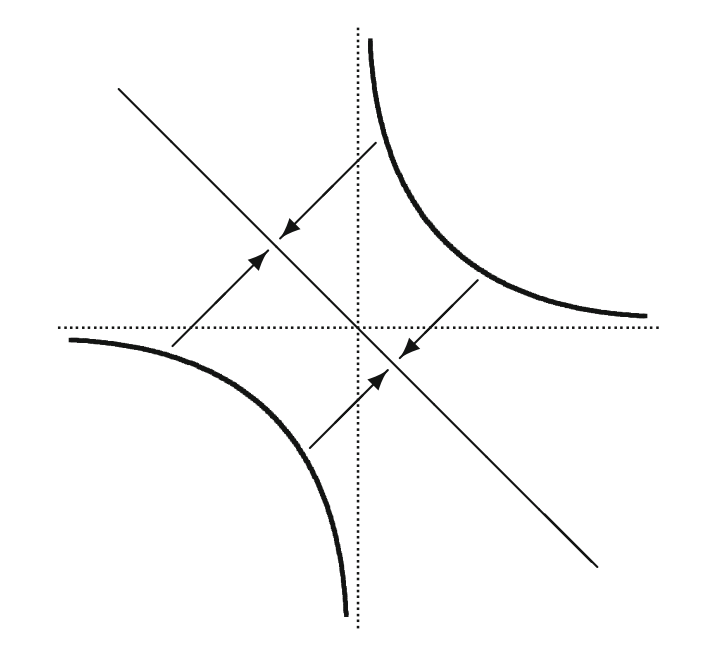
\includegraphics[scale=0.29]{Images/NoetherNormalizationLemma.png}
    \caption{A hyperbola and Noether normalization}
\end{figure}
Formally we may state as follows: If $k$ is algebraically closed and $X$ is an affine algebraic variety in $k^n$ with coordinate ring $A\ne 0$, then there exists a linear subspace $L$ of dimension $r$ in $k^n$ and a linear mapping of $k^n$ onto $L$ which maps $X$ onto $L$. Now we give an explanation on this statement.
\end{note}
\begin{problem}{\textbf{(Nullstellensatz, weak form)}}\em
Let $X$ be an affine algebraic variety in $k^n$, where $k$ is an algebraically closed field, and let $I(X)$ be the ideal of $X$ in the polynomial ring $k[t_1,\cdots,t_n]$. If $I(X)\ne (1)$ then $X$ is not empty.
\end{problem}
\begin{proof}
Let $A=k[t_1,\cdots,t_n]/I(X)$ be the coordinate ring of $X$. Then $A\ne 0$, hence by Noether's normalization lemma there exists a linear subspace $L$ of dimension $\ge 0$ in $k^n$ such that $X$ maps onto $L$. Hence $X\ne 0$.
\end{proof}
\begin{note}\par
We refer the preceding weak form of Nullstellensatz the "weaker Nullstellensatz". The "weak Nullstellensatz" usually refers to the following result: If $k$ is algebraically closed, $\mathfrak{a}$ an ideal of $k[t_1,\cdots,t_n]$, $\mathfrak{a}\ne (1)$, then $Z(\mathfrak{a})\ne 0$, where $Z(\mathfrak{a})=\{(a_1,\cdots,a_n)\in k^n:f(a_1,\cdots,a_n)=0,\forall f\in\mathfrak{a}\}$. The weak Nullstellensatz clearly implies the weaker Nullstellensatz, for taking $X=Z(\mathfrak{a})$, $I(X)\ne (1)$ implies $\mathfrak{a}\subset IZ(\mathfrak{a})$, hence $\mathfrak{a}\ne (1)$ and $X=Z(\mathfrak{a})\ne\emptyset$.\par
Another corollary (actually equivalent) of weak Nullstellensatz is that every maximal ideal in the ring $k[t_1,\cdots,t_n]$ is of the form $(t_1-a_1,\cdots,t_n-a_n)$, where $a_i\in k$.
\end{note}
\begin{problem}\textbf{(Another version of Nullstellensatz)}\em
Let $k$ be a field and let $B$ a finitely generated $k$-algebra. Suppose that $B$ is a field. Then $B$ is a finite algebraic extension of $k$.
\end{problem}
\begin{problem}\em
Deduce the result of Exercise 10.17 from Exercise 10.18.
\end{problem}